\documentclass[border=1pt,tikz,varwidth=\maxdimen]{standalone}

\usetikzlibrary{positioning,calc,trees}

\usepackage{amsmath,mathtools}

\begin{document}
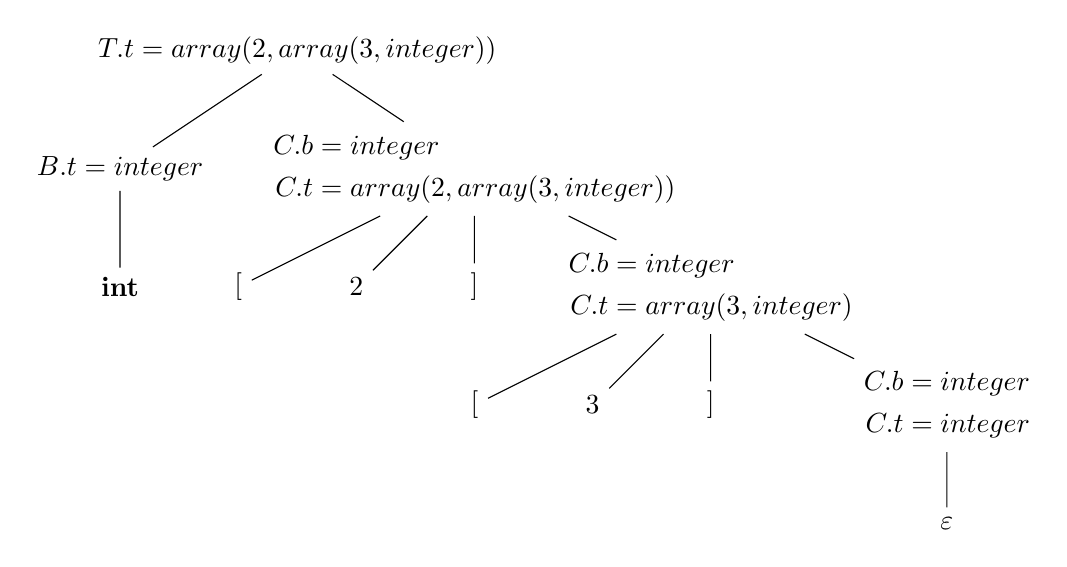
\begin{tikzpicture}
  \node{\(T.t=array(2, array(3,integer))\)}
  child {
    node {\(B.t=integer\)}
    child {
      node {\textbf{int}}
    }
  }
  child[missing]
  child[missing]
  child {
    node {\(\begin{aligned} C.b &= integer\\ C.t &= array(2,array(3,integer))\end{aligned}\)}
    child {
      node {\([\)}
    }
    child {
      node {\(2\)}
    }
    child {
      node {\(]\)}
    }
    child[missing]
    child {
      node
      {\(\begin{aligned} C.b &= integer\\ C.t &= array(3,integer)\end{aligned}\)}
      child {
        node {\([\)}
      }
      child {
        node {\(3\)}
      }
      child {
        node {\(]\)}
      }
      child[missing]
      child {
        node
        {\(\begin{aligned} C.b &= integer\\ C.t &= integer\end{aligned}\)}
        child {
          node {\(\varepsilon\)}
        }
      }
    }
  };
\end{tikzpicture}
\end{document}
